%\documentclass[]{article}
%\usepackage{mwe}
%\usepackage{tikz}

%\begin{document}

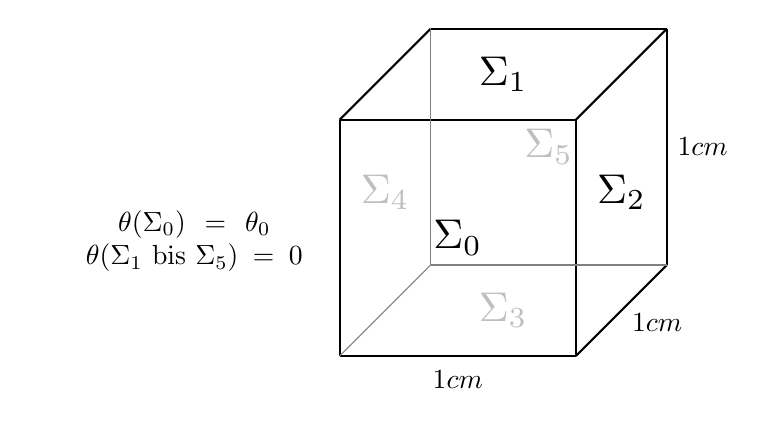
\begin{tikzpicture}
  \newcommand\x{3}
  \newcommand\h{1.5}
  \newcommand\scale{1.5}
  \newcommand\gray{50}
  \draw[thick](\x,\x,0)--(0,\x,0);
  \draw[thick](0,\x,\x)--(\x,\x,\x);
  \draw[thick](\x,\x,0)--(\x,0,0) node[midway, xshift=3ex]{$1cm$};
  \draw[thick](\x,0,\x)--(0,0,\x) node[midway, yshift=-2ex]{$1cm$};
  \draw[thick](\x,\x,\x)--(\x,0,\x);
  \draw[thick](\x,\x,\x)--(\x,0,\x);
  \draw[thick](\x,\x,\x)--(\x,0,\x);
  \draw[thick](\x,\x,\x)--(\x,0,\x);
  \draw[thick](0,\x,\x)--(0,\x,0);  
  \draw[thick](0,\x,\x)--(0,0,\x);
  \draw[thick](\x,\x,0)--(\x,\x,\x);
   \draw[thick](\x,0,0)--(\x,0,\x) node[midway, xshift=3ex, yshift=-1ex]{$1cm$};
  
  \draw[gray](\x,0,0)--(0,0,0);
  \draw[gray](0,\x,0) -- (0,0,0);
  \draw[gray](0,0,0)--(0,0,\x);
  
  \draw(\h,\h,\x) node[scale=\scale]{$\Sigma_0$};
  \draw(\h,\x,\h) node[scale=\scale]{$\Sigma_1$};
  \draw(\x,\h,\h) node[scale=\scale]{$\Sigma_2$};
  \draw[gray!\gray](\h,0,\h) node[scale=\scale]{$\Sigma_3$};
  \draw[gray!\gray](0,\h,\h) node[scale=\scale]{$\Sigma_4$};
  \draw[gray!\gray](\h,\h,0) node[scale=\scale]{$\Sigma_5$};
  \node[text width=4cm, align=center] at (-3,0.3) {$\theta(\Sigma_0) = \theta_0$ \\ $\theta(\Sigma_1$ bis $\Sigma_5) = 0$};
  
\end{tikzpicture}

%\end{document}